% Options for packages loaded elsewhere
% Options for packages loaded elsewhere
\PassOptionsToPackage{unicode}{hyperref}
\PassOptionsToPackage{hyphens}{url}
\PassOptionsToPackage{dvipsnames,svgnames,x11names}{xcolor}
%
\documentclass[
  russian,
]{article}
\usepackage{xcolor}
\usepackage[top=20mm,left=20mm,right=20mm,bottom=20mm]{geometry}
\usepackage{amsmath,amssymb}
\setcounter{secnumdepth}{5}
\usepackage{iftex}
\ifPDFTeX
  \usepackage[T1]{fontenc}
  \usepackage[utf8]{inputenc}
  \usepackage{textcomp} % provide euro and other symbols
\else % if luatex or xetex
  \usepackage{unicode-math} % this also loads fontspec
  \defaultfontfeatures{Scale=MatchLowercase}
  \defaultfontfeatures[\rmfamily]{Ligatures=TeX,Scale=1}
\fi
\usepackage{lmodern}
\ifPDFTeX\else
  % xetex/luatex font selection
  \setmainfont[]{Times New Roman}
  \setsansfont[]{Arial}
  \setmonofont[]{Courier New}
\fi
% Use upquote if available, for straight quotes in verbatim environments
\IfFileExists{upquote.sty}{\usepackage{upquote}}{}
\IfFileExists{microtype.sty}{% use microtype if available
  \usepackage[]{microtype}
  \UseMicrotypeSet[protrusion]{basicmath} % disable protrusion for tt fonts
}{}
\makeatletter
\@ifundefined{KOMAClassName}{% if non-KOMA class
  \IfFileExists{parskip.sty}{%
    \usepackage{parskip}
  }{% else
    \setlength{\parindent}{0pt}
    \setlength{\parskip}{6pt plus 2pt minus 1pt}}
}{% if KOMA class
  \KOMAoptions{parskip=half}}
\makeatother
% Make \paragraph and \subparagraph free-standing
\makeatletter
\ifx\paragraph\undefined\else
  \let\oldparagraph\paragraph
  \renewcommand{\paragraph}{
    \@ifstar
      \xxxParagraphStar
      \xxxParagraphNoStar
  }
  \newcommand{\xxxParagraphStar}[1]{\oldparagraph*{#1}\mbox{}}
  \newcommand{\xxxParagraphNoStar}[1]{\oldparagraph{#1}\mbox{}}
\fi
\ifx\subparagraph\undefined\else
  \let\oldsubparagraph\subparagraph
  \renewcommand{\subparagraph}{
    \@ifstar
      \xxxSubParagraphStar
      \xxxSubParagraphNoStar
  }
  \newcommand{\xxxSubParagraphStar}[1]{\oldsubparagraph*{#1}\mbox{}}
  \newcommand{\xxxSubParagraphNoStar}[1]{\oldsubparagraph{#1}\mbox{}}
\fi
\makeatother


\usepackage{longtable,booktabs,array}
\newcounter{none} % for unnumbered tables
\usepackage{calc} % for calculating minipage widths
% Correct order of tables after \paragraph or \subparagraph
\usepackage{etoolbox}
\makeatletter
\patchcmd\longtable{\par}{\if@noskipsec\mbox{}\fi\par}{}{}
\makeatother
% Allow footnotes in longtable head/foot
\IfFileExists{footnotehyper.sty}{\usepackage{footnotehyper}}{\usepackage{footnote}}
\makesavenoteenv{longtable}
\usepackage{graphicx}
\makeatletter
\newsavebox\pandoc@box
\newcommand*\pandocbounded[1]{% scales image to fit in text height/width
  \sbox\pandoc@box{#1}%
  \Gscale@div\@tempa{\textheight}{\dimexpr\ht\pandoc@box+\dp\pandoc@box\relax}%
  \Gscale@div\@tempb{\linewidth}{\wd\pandoc@box}%
  \ifdim\@tempb\p@<\@tempa\p@\let\@tempa\@tempb\fi% select the smaller of both
  \ifdim\@tempa\p@<\p@\scalebox{\@tempa}{\usebox\pandoc@box}%
  \else\usebox{\pandoc@box}%
  \fi%
}
% Set default figure placement to htbp
\def\fps@figure{htbp}
\makeatother



\ifLuaTeX
\usepackage[bidi=basic,shorthands=off,provide=*]{babel}
\else
\usepackage[bidi=default,shorthands=off,provide=*]{babel}
\fi
\ifPDFTeX
\else
\babelfont{rm}[]{Times New Roman}
\fi
\ifLuaTeX
  \usepackage{selnolig} % disable illegal ligatures
\fi


\setlength{\emergencystretch}{3em} % prevent overfull lines

\providecommand{\tightlist}{%
  \setlength{\itemsep}{0pt}\setlength{\parskip}{0pt}}



 


\makeatletter
\@ifpackageloaded{tcolorbox}{}{\usepackage[skins,breakable]{tcolorbox}}
\@ifpackageloaded{fontawesome5}{}{\usepackage{fontawesome5}}
\definecolor{quarto-callout-color}{HTML}{909090}
\definecolor{quarto-callout-note-color}{HTML}{0758E5}
\definecolor{quarto-callout-important-color}{HTML}{CC1914}
\definecolor{quarto-callout-warning-color}{HTML}{EB9113}
\definecolor{quarto-callout-tip-color}{HTML}{00A047}
\definecolor{quarto-callout-caution-color}{HTML}{FC5300}
\definecolor{quarto-callout-color-frame}{HTML}{acacac}
\definecolor{quarto-callout-note-color-frame}{HTML}{4582ec}
\definecolor{quarto-callout-important-color-frame}{HTML}{d9534f}
\definecolor{quarto-callout-warning-color-frame}{HTML}{f0ad4e}
\definecolor{quarto-callout-tip-color-frame}{HTML}{02b875}
\definecolor{quarto-callout-caution-color-frame}{HTML}{fd7e14}
\makeatother
\makeatletter
\@ifpackageloaded{caption}{}{\usepackage{caption}}
\AtBeginDocument{%
\ifdefined\contentsname
  \renewcommand*\contentsname{Содержание}
\else
  \newcommand\contentsname{Содержание}
\fi
\ifdefined\listfigurename
  \renewcommand*\listfigurename{Список Иллюстраций}
\else
  \newcommand\listfigurename{Список Иллюстраций}
\fi
\ifdefined\listtablename
  \renewcommand*\listtablename{Список Таблиц}
\else
  \newcommand\listtablename{Список Таблиц}
\fi
\ifdefined\figurename
  \renewcommand*\figurename{Рисунок}
\else
  \newcommand\figurename{Рисунок}
\fi
\ifdefined\tablename
  \renewcommand*\tablename{Таблица}
\else
  \newcommand\tablename{Таблица}
\fi
}
\@ifpackageloaded{float}{}{\usepackage{float}}
\floatstyle{ruled}
\@ifundefined{c@chapter}{\newfloat{codelisting}{h}{lop}}{\newfloat{codelisting}{h}{lop}[chapter]}
\floatname{codelisting}{Список}
\newcommand*\listoflistings{\listof{codelisting}{Список Каталогов}}
\makeatother
\makeatletter
\makeatother
\makeatletter
\@ifpackageloaded{caption}{}{\usepackage{caption}}
\@ifpackageloaded{subcaption}{}{\usepackage{subcaption}}
\makeatother
\usepackage{bookmark}
\IfFileExists{xurl.sty}{\usepackage{xurl}}{} % add URL line breaks if available
\urlstyle{same}
% fallback for those not using the hyperref driver hyperxmp:
\makeatletter
\@ifundefined{xmpquote}{\newcommand{\xmpquote}[1]{#1}}{}
\makeatother
\hypersetup{
  pdftitle={Задачи по Эконометрике-1: Категориальные регрессоры и структурные сдвиги},
  pdfauthor={Н. В. Артамонов, А. Н. Лата (МГИМО МИД России)},
  pdflang={ru},
  colorlinks=true,
  linkcolor={blue},
  filecolor={Maroon},
  citecolor={Blue},
  urlcolor={Blue},
  pdfcreator={LaTeX via pandoc}}


\title{Задачи по Эконометрике-1: Категориальные регрессоры и структурные
сдвиги}
\author{Н. В. Артамонов, А. Н. Лата (МГИМО МИД России)}
\date{}
\begin{document}
\maketitle

\renewcommand*\contentsname{Содержание}
{
\setcounter{tocdepth}{3}
\tableofcontents
}

\begin{tcolorbox}[enhanced jigsaw, arc=.35mm, bottomrule=.15mm, bottomtitle=1mm, breakable, colback=white, colbacktitle=quarto-callout-important-color!10!white, colframe=quarto-callout-important-color-frame, coltitle=black, left=2mm, leftrule=.75mm, opacityback=0, opacitybacktitle=0.6, rightrule=.15mm, title=\textcolor{quarto-callout-important-color}{\faExclamation}\hspace{0.5em}{Важно}, titlerule=0mm, toprule=.15mm, toptitle=1mm]

\begin{itemize}
\tightlist
\item
  Логарифм натуральный; константа включается в модель по умолчанию.
\item
  Данные лежат в \texttt{datasets/}, описание переменных --- в
  \texttt{datasets/data-description.md}.
\item
  Ответы округляются до 2-х десятичных знаков, если в задаче не сказано
  иное; ответы считаются по неокруглённым оценкам.
\item
  Коэффициенты подписаны так, как их печатает statsmodels:
  \texttt{Intercept} --- константа, \texttt{np.log(x)} --- \(\log x\),
  \texttt{I(x\ **\ 2)} --- \(x^2\), \texttt{x:d} --- произведение
  \texttt{x} и \texttt{d}.
\item
  \texttt{x{[}T.a{]}} --- бинарная переменная для категории \texttt{a}
  категориального регрессора \texttt{x}. Например,
  \texttt{colour{[}T.E{]}} равна 1 для бриллиантов цвета E и 0 для
  остальных. У базовой категории своей строки нет; она названа в условии
  задачи.
\item
  В таблицах раздела «Структурные сдвиги» в скобках --- неробастные
  стандартные ошибки.
\end{itemize}

\end{tcolorbox}

\section{Категориальные
регрессоры}\label{ux43aux430ux442ux435ux433ux43eux440ux438ux430ux43bux44cux43dux44bux435-ux440ux435ux433ux440ux435ux441ux441ux43eux440ux44b}

\subsection{diamond equation \#1}\label{diamond-equation-1}

Набор данных \texttt{Diamond}: \texttt{price} --- цена, сингапурские
доллары; \texttt{carat} --- масса, караты; \texttt{colour} --- цвет от D
(лучший) до I; \texttt{clarity} --- чистота; \texttt{certification} ---
организация, выдавшая сертификат (GIA, HRD, IGI).

\textbf{Описательные статистики}

Для набора данных \texttt{Diamond} вычислите описательные статистики
количественных переменных (\texttt{df.describe()}) и число наблюдений по
уровням категориальных регрессоров
(\texttt{df{[}\textquotesingle{}colour\textquotesingle{}{]}.value\_counts()}).

{\def\LTcaptype{none} % do not increment counter
\begin{longtable}[]{@{}rrr@{}}
\toprule\noalign{}
& carat & price \\
\midrule\noalign{}
\endhead
\bottomrule\noalign{}
\endlastfoot
count & 308 & 308 \\
mean & 0.6309 & 5019 \\
std & 0.2772 & 3403 \\
min & 0.1800 & 638 \\
25\% & 0.3500 & 1625 \\
50\% & 0.6200 & 4215 \\
75\% & 0.8500 & 7446 \\
max & 1.1000 & 16008 \\
\end{longtable}
}

{\def\LTcaptype{none} % do not increment counter
\begin{longtable}[]{@{}lrrrrrr@{}}
\toprule\noalign{}
& D & E & F & G & H & I \\
\midrule\noalign{}
\endhead
\bottomrule\noalign{}
\endlastfoot
colour: число наблюдений & 16 & 44 & 82 & 65 & 61 & 40 \\
\end{longtable}
}

{\def\LTcaptype{none} % do not increment counter
\begin{longtable}[]{@{}lrrrrr@{}}
\toprule\noalign{}
& IF & VS1 & VS2 & VVS1 & VVS2 \\
\midrule\noalign{}
\endhead
\bottomrule\noalign{}
\endlastfoot
clarity: число наблюдений & 44 & 81 & 53 & 52 & 78 \\
\end{longtable}
}

{\def\LTcaptype{none} % do not increment counter
\begin{longtable}[]{@{}lrrr@{}}
\toprule\noalign{}
& GIA & HRD & IGI \\
\midrule\noalign{}
\endhead
\bottomrule\noalign{}
\endlastfoot
certification: число наблюдений & 151 & 79 & 78 \\
\end{longtable}
}

\textbf{Регрессии}

Для набора данных \texttt{Diamond} рассмотрим несколько линейных
регрессий.

\begin{enumerate}
\def\labelenumi{\arabic{enumi}.}
\tightlist
\item
  \texttt{np.log(price)\ \textasciitilde{}\ carat\ +\ I(carat**2)\ +\ colour}
\item
  \texttt{np.log(price)\ \textasciitilde{}\ carat\ +\ I(carat**2)\ +\ certification}
\item
  \texttt{np.log(price)\ \textasciitilde{}\ carat\ +\ I(carat**2)\ +\ colour\ +\ certification}
\end{enumerate}

Базовые категории: \texttt{colour} --- D, \texttt{certification} ---
GIA.

Оцените регрессии и дайте интерпретацию коэффициентам для категориальных
регрессоров. Интерпретацию дайте в процентах: приближённо
(\(100\cdot\beta\)) и точно (\(100\cdot(e^{\beta}-1)\)). \textbf{Ответ
округлите до 2-х десятичных знаков.}

Результаты оценивания

\textbf{Модель 1}

{\def\LTcaptype{none} % do not increment counter
\begin{longtable}[]{@{}lr@{}}
\toprule\noalign{}
Переменная & Оценка \\
\midrule\noalign{}
\endhead
\bottomrule\noalign{}
\endlastfoot
Intercept & 5.98 \\
colour{[}T.E{]} & -0.07 \\
colour{[}T.F{]} & -0.14 \\
colour{[}T.G{]} & -0.21 \\
colour{[}T.H{]} & -0.30 \\
colour{[}T.I{]} & -0.40 \\
carat & 5.40 \\
I(carat ** 2) & -1.98 \\
\end{longtable}
}

Модель была подогнана по 308 наблюдениям.

\textbf{Модель 2}

{\def\LTcaptype{none} % do not increment counter
\begin{longtable}[]{@{}lr@{}}
\toprule\noalign{}
Переменная & Оценка \\
\midrule\noalign{}
\endhead
\bottomrule\noalign{}
\endlastfoot
Intercept & 5.69 \\
certification{[}T.HRD{]} & 0.03 \\
certification{[}T.IGI{]} & 0.07 \\
carat & 5.65 \\
I(carat ** 2) & -2.19 \\
\end{longtable}
}

Модель была подогнана по 308 наблюдениям.

\textbf{Модель 3}

{\def\LTcaptype{none} % do not increment counter
\begin{longtable}[]{@{}lr@{}}
\toprule\noalign{}
Переменная & Оценка \\
\midrule\noalign{}
\endhead
\bottomrule\noalign{}
\endlastfoot
Intercept & 5.87 \\
colour{[}T.E{]} & -0.08 \\
colour{[}T.F{]} & -0.15 \\
colour{[}T.G{]} & -0.23 \\
colour{[}T.H{]} & -0.31 \\
colour{[}T.I{]} & -0.41 \\
certification{[}T.HRD{]} & 0.04 \\
certification{[}T.IGI{]} & 0.09 \\
carat & 5.67 \\
I(carat ** 2) & -2.15 \\
\end{longtable}
}

Модель была подогнана по 308 наблюдениям.

\begin{figure}

\centering{

\pandocbounded{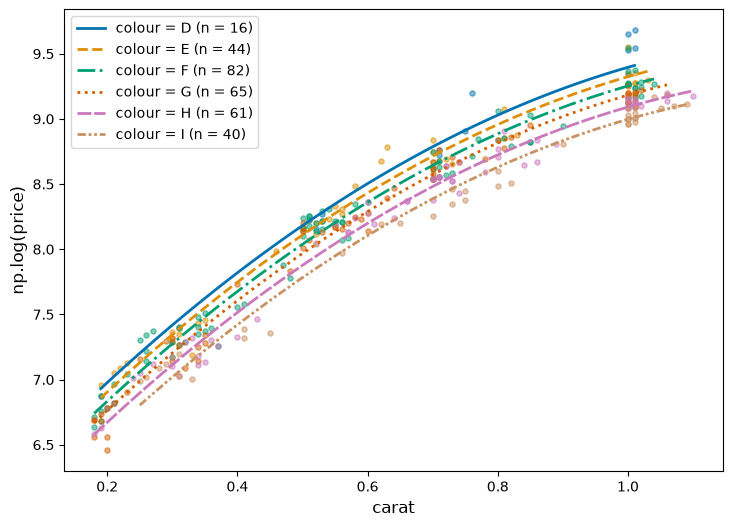
\includegraphics[keepaspectratio]{list05-specification_files/figure-pdf/fig-diamond-colour-output-1.png}}

}

\caption{\label{fig-diamond-colour}np.log(price) и carat по категориям
colour (Diamond): категориальный регрессор сдвигает кривую параллельно}

\end{figure}%

\begin{tcolorbox}[enhanced jigsaw, arc=.35mm, bottomrule=.15mm, bottomtitle=1mm, breakable, colback=white, colbacktitle=quarto-callout-tip-color!10!white, colframe=quarto-callout-tip-color-frame, coltitle=black, left=2mm, leftrule=.75mm, opacityback=0, opacitybacktitle=0.6, rightrule=.15mm, title=\textcolor{quarto-callout-tip-color}{\faLightbulb}\hspace{0.5em}{Ответ}, titlerule=0mm, toprule=.15mm, toptitle=1mm]

\textbf{Модель 1.} Базовая категория --- цвет D (лучший). При той же
массе бриллиант дешевле бриллианта цвета D: E --- на 7 \% (7.0 \%), F
--- на 14 \% (13.3 \%), G --- на 21 \% (19.2 \%), H --- на 30 \% (26.3
\%), I --- на 40 \% (32.9 \%). Первое число --- приближённая оценка
\(100\cdot\beta\), в скобках --- точная \(100\cdot(e^{\beta}-1)\); чем
больше \(\lvert\beta\rvert\), тем сильнее они расходятся. Коэффициент
при \texttt{colour{[}T.E{]}} --- вертикальный сдвиг кривой относительно
кривой цвета D (Рисунок~\ref{fig-diamond-colour}).

\textbf{Модель 2.} Базовая категория --- сертификат GIA. При той же
массе бриллиант дороже бриллианта с сертификатом GIA: HRD --- на 3 \%
(3.2 \%), IGI --- на 7 \% (7.0 \%).

\end{tcolorbox}

\subsection{diamond equation \#2}\label{diamond-equation-2}

Набор данных \texttt{diamonds}: \texttt{price} --- цена, долл. США;
\texttt{carat} --- масса, караты; \texttt{cut} --- качество огранки от
Fair (худшее) до Ideal; \texttt{color} --- цвет от D (лучший) до J;
\texttt{clarity} --- чистота; \texttt{x}, \texttt{y}, \texttt{z} ---
длина, ширина, высота в мм.

\textbf{Описательные статистики}

Для набора данных \texttt{diamonds} вычислите описательные статистики
количественных переменных (\texttt{df.describe()}) и число наблюдений по
уровням категориальных регрессоров
(\texttt{df{[}\textquotesingle{}cut\textquotesingle{}{]}.value\_counts()}).

Какие значения в таблице описательных статистик выглядят ошибочными?
Сколько таких наблюдений?

{\def\LTcaptype{none} % do not increment counter
\begin{longtable}[]{@{}
  >{\raggedleft\arraybackslash}p{(\linewidth - 14\tabcolsep) * \real{0.1045}}
  >{\raggedleft\arraybackslash}p{(\linewidth - 14\tabcolsep) * \real{0.1343}}
  >{\raggedleft\arraybackslash}p{(\linewidth - 14\tabcolsep) * \real{0.1343}}
  >{\raggedleft\arraybackslash}p{(\linewidth - 14\tabcolsep) * \real{0.1343}}
  >{\raggedleft\arraybackslash}p{(\linewidth - 14\tabcolsep) * \real{0.1343}}
  >{\raggedleft\arraybackslash}p{(\linewidth - 14\tabcolsep) * \real{0.1194}}
  >{\raggedleft\arraybackslash}p{(\linewidth - 14\tabcolsep) * \real{0.1194}}
  >{\raggedleft\arraybackslash}p{(\linewidth - 14\tabcolsep) * \real{0.1194}}@{}}
\toprule\noalign{}
\begin{minipage}[b]{\linewidth}\raggedleft
\end{minipage} & \begin{minipage}[b]{\linewidth}\raggedleft
carat
\end{minipage} & \begin{minipage}[b]{\linewidth}\raggedleft
depth
\end{minipage} & \begin{minipage}[b]{\linewidth}\raggedleft
table
\end{minipage} & \begin{minipage}[b]{\linewidth}\raggedleft
price
\end{minipage} & \begin{minipage}[b]{\linewidth}\raggedleft
x
\end{minipage} & \begin{minipage}[b]{\linewidth}\raggedleft
y
\end{minipage} & \begin{minipage}[b]{\linewidth}\raggedleft
z
\end{minipage} \\
\midrule\noalign{}
\endhead
\bottomrule\noalign{}
\endlastfoot
count & 53940 & 53940 & 53940 & 53940 & 53940 & 53940 & 53940 \\
mean & 0.7979 & 61.75 & 57.46 & 3933 & 5.731 & 5.735 & 3.539 \\
std & 0.4740 & 1.43 & 2.23 & 3989 & 1.122 & 1.142 & 0.706 \\
min & 0.2000 & 43.00 & 43.00 & 326 & 0.000 & 0.000 & 0.000 \\
25\% & 0.4000 & 61.00 & 56.00 & 950 & 4.710 & 4.720 & 2.910 \\
50\% & 0.7000 & 61.80 & 57.00 & 2401 & 5.700 & 5.710 & 3.530 \\
75\% & 1.0400 & 62.50 & 59.00 & 5324 & 6.540 & 6.540 & 4.040 \\
max & 5.0100 & 79.00 & 95.00 & 18823 & 10.740 & 58.900 & 31.800 \\
\end{longtable}
}

{\def\LTcaptype{none} % do not increment counter
\begin{longtable}[]{@{}
  >{\raggedright\arraybackslash}p{(\linewidth - 10\tabcolsep) * \real{0.3194}}
  >{\raggedleft\arraybackslash}p{(\linewidth - 10\tabcolsep) * \real{0.1111}}
  >{\raggedleft\arraybackslash}p{(\linewidth - 10\tabcolsep) * \real{0.1111}}
  >{\raggedleft\arraybackslash}p{(\linewidth - 10\tabcolsep) * \real{0.1806}}
  >{\raggedleft\arraybackslash}p{(\linewidth - 10\tabcolsep) * \real{0.1528}}
  >{\raggedleft\arraybackslash}p{(\linewidth - 10\tabcolsep) * \real{0.1250}}@{}}
\toprule\noalign{}
\begin{minipage}[b]{\linewidth}\raggedright
\end{minipage} & \begin{minipage}[b]{\linewidth}\raggedleft
Fair
\end{minipage} & \begin{minipage}[b]{\linewidth}\raggedleft
Good
\end{minipage} & \begin{minipage}[b]{\linewidth}\raggedleft
Very Good
\end{minipage} & \begin{minipage}[b]{\linewidth}\raggedleft
Premium
\end{minipage} & \begin{minipage}[b]{\linewidth}\raggedleft
Ideal
\end{minipage} \\
\midrule\noalign{}
\endhead
\bottomrule\noalign{}
\endlastfoot
cut: число наблюдений & 1610 & 4906 & 12082 & 13791 & 21551 \\
\end{longtable}
}

{\def\LTcaptype{none} % do not increment counter
\begin{longtable}[]{@{}
  >{\raggedright\arraybackslash}p{(\linewidth - 14\tabcolsep) * \real{0.3676}}
  >{\raggedleft\arraybackslash}p{(\linewidth - 14\tabcolsep) * \real{0.0882}}
  >{\raggedleft\arraybackslash}p{(\linewidth - 14\tabcolsep) * \real{0.0882}}
  >{\raggedleft\arraybackslash}p{(\linewidth - 14\tabcolsep) * \real{0.0882}}
  >{\raggedleft\arraybackslash}p{(\linewidth - 14\tabcolsep) * \real{0.1029}}
  >{\raggedleft\arraybackslash}p{(\linewidth - 14\tabcolsep) * \real{0.0882}}
  >{\raggedleft\arraybackslash}p{(\linewidth - 14\tabcolsep) * \real{0.0882}}
  >{\raggedleft\arraybackslash}p{(\linewidth - 14\tabcolsep) * \real{0.0882}}@{}}
\toprule\noalign{}
\begin{minipage}[b]{\linewidth}\raggedright
\end{minipage} & \begin{minipage}[b]{\linewidth}\raggedleft
D
\end{minipage} & \begin{minipage}[b]{\linewidth}\raggedleft
E
\end{minipage} & \begin{minipage}[b]{\linewidth}\raggedleft
F
\end{minipage} & \begin{minipage}[b]{\linewidth}\raggedleft
G
\end{minipage} & \begin{minipage}[b]{\linewidth}\raggedleft
H
\end{minipage} & \begin{minipage}[b]{\linewidth}\raggedleft
I
\end{minipage} & \begin{minipage}[b]{\linewidth}\raggedleft
J
\end{minipage} \\
\midrule\noalign{}
\endhead
\bottomrule\noalign{}
\endlastfoot
color: число наблюдений & 6775 & 9797 & 9542 & 11292 & 8304 & 5422 &
2808 \\
\end{longtable}
}

{\def\LTcaptype{none} % do not increment counter
\begin{longtable}[]{@{}
  >{\raggedright\arraybackslash}p{(\linewidth - 16\tabcolsep) * \real{0.3253}}
  >{\raggedleft\arraybackslash}p{(\linewidth - 16\tabcolsep) * \real{0.0723}}
  >{\raggedleft\arraybackslash}p{(\linewidth - 16\tabcolsep) * \real{0.0843}}
  >{\raggedleft\arraybackslash}p{(\linewidth - 16\tabcolsep) * \real{0.0843}}
  >{\raggedleft\arraybackslash}p{(\linewidth - 16\tabcolsep) * \real{0.0843}}
  >{\raggedleft\arraybackslash}p{(\linewidth - 16\tabcolsep) * \real{0.0843}}
  >{\raggedleft\arraybackslash}p{(\linewidth - 16\tabcolsep) * \real{0.0964}}
  >{\raggedleft\arraybackslash}p{(\linewidth - 16\tabcolsep) * \real{0.0964}}
  >{\raggedleft\arraybackslash}p{(\linewidth - 16\tabcolsep) * \real{0.0723}}@{}}
\toprule\noalign{}
\begin{minipage}[b]{\linewidth}\raggedright
\end{minipage} & \begin{minipage}[b]{\linewidth}\raggedleft
I1
\end{minipage} & \begin{minipage}[b]{\linewidth}\raggedleft
SI2
\end{minipage} & \begin{minipage}[b]{\linewidth}\raggedleft
SI1
\end{minipage} & \begin{minipage}[b]{\linewidth}\raggedleft
VS2
\end{minipage} & \begin{minipage}[b]{\linewidth}\raggedleft
VS1
\end{minipage} & \begin{minipage}[b]{\linewidth}\raggedleft
VVS2
\end{minipage} & \begin{minipage}[b]{\linewidth}\raggedleft
VVS1
\end{minipage} & \begin{minipage}[b]{\linewidth}\raggedleft
IF
\end{minipage} \\
\midrule\noalign{}
\endhead
\bottomrule\noalign{}
\endlastfoot
clarity: число наблюдений & 741 & 9194 & 13065 & 12258 & 8171 & 5066 &
3655 & 1790 \\
\end{longtable}
}

\begin{tcolorbox}[enhanced jigsaw, arc=.35mm, bottomrule=.15mm, bottomtitle=1mm, breakable, colback=white, colbacktitle=quarto-callout-tip-color!10!white, colframe=quarto-callout-tip-color-frame, coltitle=black, left=2mm, leftrule=.75mm, opacityback=0, opacitybacktitle=0.6, rightrule=.15mm, title=\textcolor{quarto-callout-tip-color}{\faLightbulb}\hspace{0.5em}{Ответ}, titlerule=0mm, toprule=.15mm, toptitle=1mm]

Нулевые минимумы размеров \texttt{x}, \texttt{y}, \texttt{z} (число
наблюдений с нулём: \texttt{x} --- 8, \texttt{y} --- 7, \texttt{z} ---
20) и максимумы \texttt{y} = 58.9 мм, \texttt{z} = 31.8 мм при третьих
квартилях 6.54 и 4.04 мм.

\end{tcolorbox}

\textbf{Регрессии}

Для набора данных \texttt{diamonds} рассмотрим несколько линейных
регрессий.

\begin{enumerate}
\def\labelenumi{\arabic{enumi}.}
\tightlist
\item
  \texttt{np.log(price)\ \textasciitilde{}\ carat\ +\ I(carat**2)\ +\ cut\ +\ x\ +\ y\ +\ z}
\item
  \texttt{np.log(price)\ \textasciitilde{}\ carat\ +\ I(carat**2)\ +\ color\ +\ x\ +\ y\ +\ z}
\item
  \texttt{np.log(price)\ \textasciitilde{}\ carat\ +\ I(carat**2)\ +\ color\ +\ cut\ +\ x\ +\ y\ +\ z}
\end{enumerate}

Базовые категории: \texttt{cut} --- Fair, \texttt{color} --- D.

Оцените регрессии и дайте интерпретацию коэффициентам для категориальных
регрессоров. Интерпретацию дайте в процентах: приближённо
(\(100\cdot\beta\)) и точно (\(100\cdot(e^{\beta}-1)\)). \textbf{Ответ
округлите до 2-х десятичных знаков.}

Результаты оценивания

\textbf{Модель 1}

{\def\LTcaptype{none} % do not increment counter
\begin{longtable}[]{@{}lr@{}}
\toprule\noalign{}
Переменная & Оценка \\
\midrule\noalign{}
\endhead
\bottomrule\noalign{}
\endlastfoot
Intercept & 3.80 \\
cut{[}T.Good{]} & 0.12 \\
cut{[}T.Very Good{]} & 0.17 \\
cut{[}T.Premium{]} & 0.16 \\
cut{[}T.Ideal{]} & 0.24 \\
carat & 2.37 \\
I(carat ** 2) & -0.64 \\
x & 0.38 \\
y & 0.02 \\
z & 0.06 \\
\end{longtable}
}

Модель была подогнана по 53940 наблюдениям.

\textbf{Модель 2}

{\def\LTcaptype{none} % do not increment counter
\begin{longtable}[]{@{}lr@{}}
\toprule\noalign{}
Переменная & Оценка \\
\midrule\noalign{}
\endhead
\bottomrule\noalign{}
\endlastfoot
Intercept & 4.08 \\
color{[}T.E{]} & -0.03 \\
color{[}T.F{]} & -0.04 \\
color{[}T.G{]} & -0.07 \\
color{[}T.H{]} & -0.21 \\
color{[}T.I{]} & -0.30 \\
color{[}T.J{]} & -0.43 \\
carat & 2.35 \\
I(carat ** 2) & -0.61 \\
x & 0.38 \\
y & 0.03 \\
z & 0.05 \\
\end{longtable}
}

Модель была подогнана по 53940 наблюдениям.

\textbf{Модель 3}

{\def\LTcaptype{none} % do not increment counter
\begin{longtable}[]{@{}lr@{}}
\toprule\noalign{}
Переменная & Оценка \\
\midrule\noalign{}
\endhead
\bottomrule\noalign{}
\endlastfoot
Intercept & 3.99 \\
color{[}T.E{]} & -0.03 \\
color{[}T.F{]} & -0.04 \\
color{[}T.G{]} & -0.07 \\
color{[}T.H{]} & -0.21 \\
color{[}T.I{]} & -0.31 \\
color{[}T.J{]} & -0.43 \\
cut{[}T.Good{]} & 0.12 \\
cut{[}T.Very Good{]} & 0.18 \\
cut{[}T.Premium{]} & 0.16 \\
cut{[}T.Ideal{]} & 0.25 \\
carat & 2.54 \\
I(carat ** 2) & -0.65 \\
x & 0.34 \\
y & 0.01 \\
z & 0.06 \\
\end{longtable}
}

Модель была подогнана по 53940 наблюдениям.

\begin{tcolorbox}[enhanced jigsaw, arc=.35mm, bottomrule=.15mm, bottomtitle=1mm, breakable, colback=white, colbacktitle=quarto-callout-tip-color!10!white, colframe=quarto-callout-tip-color-frame, coltitle=black, left=2mm, leftrule=.75mm, opacityback=0, opacitybacktitle=0.6, rightrule=.15mm, title=\textcolor{quarto-callout-tip-color}{\faLightbulb}\hspace{0.5em}{Ответ}, titlerule=0mm, toprule=.15mm, toptitle=1mm]

\textbf{Модель 1.} Базовая категория --- огранка Fair (худшая). При тех
же массе и размерах бриллиант дороже бриллианта с огранкой Fair: Good
--- на 12 \% (12.3 \%), Very Good --- на 17 \% (18.9 \%), Premium --- на
16 \% (16.8 \%), Ideal --- на 24 \% (27.7 \%). Первое число ---
приближённая оценка \(100\cdot\beta\), в скобках --- точная
\(100\cdot(e^{\beta}-1)\).

\textbf{Модель 2.} Базовая категория --- цвет D (лучший). При тех же
массе и размерах бриллиант дешевле бриллианта цвета D: E --- на 3 \%
(3.1 \%), F --- на 4 \% (3.9 \%), G --- на 7 \% (6.5 \%), H --- на 21 \%
(18.9 \%), I --- на 30 \% (26.2 \%), J --- на 43 \% (35.2 \%).

\end{tcolorbox}

\section{Структурные
сдвиги}\label{ux441ux442ux440ux443ux43aux442ux443ux440ux43dux44bux435-ux441ux434ux432ux438ux433ux438}

\subsection{Рисунки: sleep по группам
south}\label{ux440ux438ux441ux443ux43dux43aux438-sleep-ux43fux43e-ux433ux440ux443ux43fux43fux430ux43c-south}

Набор данных \texttt{sleep75}: \texttt{sleep}, \texttt{totwrk} --- сон и
работа, минут в неделю; \texttt{age} --- возраст, лет; \texttt{smsa} = 1
--- живёт в крупной городской агломерации; \texttt{south} = 1 --- южные
штаты; \texttt{male} = 1 --- мужчина.

Рисунок~\ref{fig-sleep-totwrk} --- диаграмма рассеяния \texttt{sleep} и
\texttt{totwrk} (набор данных \texttt{sleep75}) и три прямые МНК: по
полной выборке, по наблюдениям с \texttt{south\ =\ 0} и с
\texttt{south\ =\ 1}. Рисунок~\ref{fig-sleep-age} --- то же для
регрессии \textbf{sleep на age, I(age**2)}.

\begin{figure}

\centering{

\pandocbounded{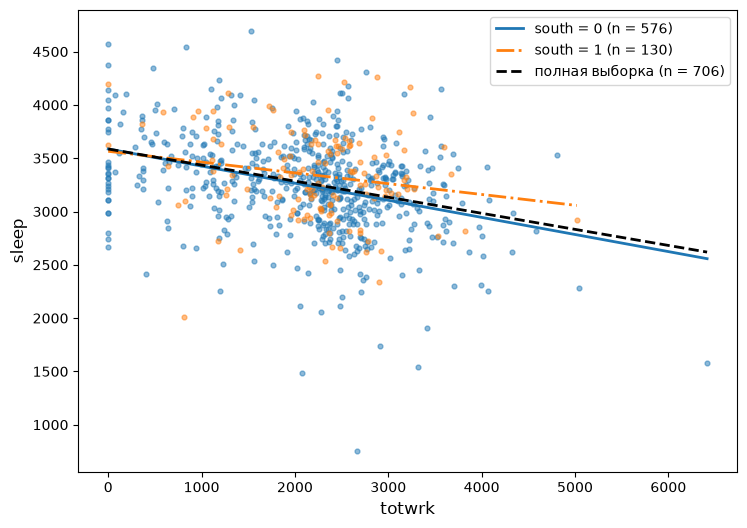
\includegraphics[keepaspectratio]{list05-specification_files/figure-pdf/fig-sleep-totwrk-output-1.png}}

}

\caption{\label{fig-sleep-totwrk}sleep на totwrk: подгонка по полной
выборке и отдельно для south = 0 и south = 1}

\end{figure}%

\begin{figure}

\centering{

\pandocbounded{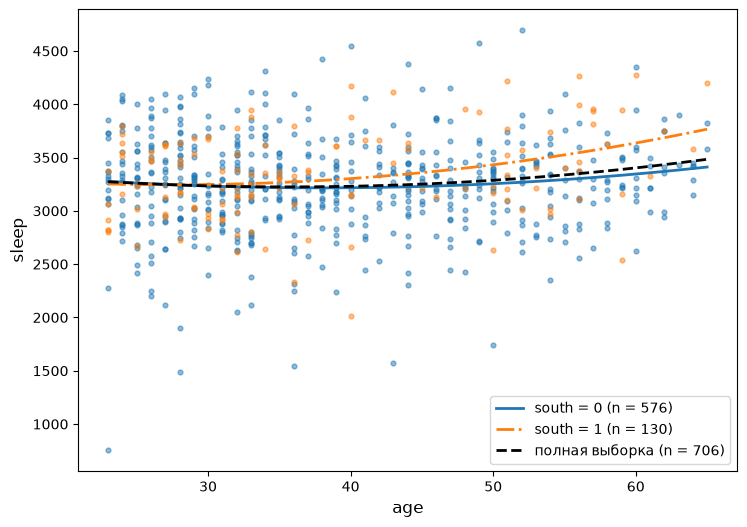
\includegraphics[keepaspectratio]{list05-specification_files/figure-pdf/fig-sleep-age-output-1.png}}

}

\caption{\label{fig-sleep-age}sleep на age, I(age**2): подгонка по
полной выборке и отдельно для south = 0 и south = 1}

\end{figure}%

Чем различаются прямые для \texttt{south\ =\ 0} и \texttt{south\ =\ 1}
(Рисунок~\ref{fig-sleep-totwrk}): сдвигом, наклоном или и тем и другим?

Почему линия полной выборки почти совпадает с линией
\texttt{south\ =\ 0}?

Какими регрессорами нужно дополнить модель \textbf{sleep на totwrk},
чтобы одна регрессия дала обе прямые?

\begin{tcolorbox}[enhanced jigsaw, arc=.35mm, bottomrule=.15mm, bottomtitle=1mm, breakable, colback=white, colbacktitle=quarto-callout-tip-color!10!white, colframe=quarto-callout-tip-color-frame, coltitle=black, left=2mm, leftrule=.75mm, opacityback=0, opacitybacktitle=0.6, rightrule=.15mm, title=\textcolor{quarto-callout-tip-color}{\faLightbulb}\hspace{0.5em}{Ответ}, titlerule=0mm, toprule=.15mm, toptitle=1mm]

Различается в основном наклон: -0.160 при \texttt{south\ =\ 0} и -0.101
при \texttt{south\ =\ 1}; константы близки (3586.7 и 3564.9). На группу
\texttt{south\ =\ 0} приходится 576 наблюдений из 706, поэтому она
определяет линию полной выборки. Модель нужно дополнить регрессорами
\texttt{south} (сдвиг константы) и \texttt{totwrk:south} (сдвиг
наклона).

\end{tcolorbox}

\subsection{sleep equation \#1}\label{sleep-equation-1}

Для набора данных \texttt{sleep75} рассмотрим регрессию \textbf{sleep на
totwrk, age, smsa}: исходную (1) и со структурными сдвигами относительно
бинарной переменной \texttt{male} (1 --- мужчина) (2):

\texttt{sleep\ \textasciitilde{}\ totwrk\ +\ age\ +\ smsa\ +\ male\ +\ totwrk:male\ +\ age:male\ +\ smsa:male}

Результаты оценивания

{\def\LTcaptype{none} % do not increment counter
\begin{longtable}[]{@{}lcc@{}}
\toprule\noalign{}
& (1) & (2) \\
\midrule\noalign{}
\endhead
\bottomrule\noalign{}
\endlastfoot
Dep. Variable & sleep & sleep \\
Intercept & 3498.670 & 3486.973 \\
& (69.133) & (92.418) \\
totwrk & -0.150*** & -0.143*** \\
& (0.017) & (0.026) \\
age & 2.997** & 1.704 \\
& (1.393) & (2.085) \\
smsa & -73.501** & -56.649 \\
& (32.219) & (48.902) \\
male & & 135.200 \\
& & (143.832) \\
totwrk:male & & -0.045 \\
& & (0.036) \\
age:male & & 1.500 \\
& & (2.825) \\
smsa:male & & -34.735 \\
& & (64.938) \\
R-squared & 0.115 & 0.126 \\
R-squared Adj. & 0.112 & 0.117 \\
F Statistic & 30.527*** & 14.387*** \\
Observations & 706 & 706 \\
Residual Std. Error & 418.877 & 417.530 \\
\end{longtable}
}

\emph{Signif. codes:} \texttt{***} \(p<0.01\), \texttt{**} \(p<0.05\),
\texttt{*} \(p<0.1\). В скобках --- неробастные стандартные ошибки.

Для регрессии (2) выпишите оценённое уравнение отдельно для
\texttt{male\ =\ 0} и для \texttt{male\ =\ 1}. Что показывают
коэффициенты при \texttt{male} и при \texttt{age:male}? \textbf{Ответ
округлите до 3-х десятичных знаков.}

\begin{tcolorbox}[enhanced jigsaw, arc=.35mm, bottomrule=.15mm, bottomtitle=1mm, breakable, colback=white, colbacktitle=quarto-callout-tip-color!10!white, colframe=quarto-callout-tip-color-frame, coltitle=black, left=2mm, leftrule=.75mm, opacityback=0, opacitybacktitle=0.6, rightrule=.15mm, title=\textcolor{quarto-callout-tip-color}{\faLightbulb}\hspace{0.5em}{Ответ}, titlerule=0mm, toprule=.15mm, toptitle=1mm]

\begin{itemize}
\tightlist
\item
  \texttt{male\ =\ 0}: sleep = 3486.973 − 0.143·totwrk + 1.704·age −
  56.649·smsa
\item
  \texttt{male\ =\ 1}: sleep = 3622.172 − 0.188·totwrk + 3.204·age −
  91.384·smsa
\end{itemize}

Коэффициент при \texttt{male} (135.200) --- разность констант двух
уравнений. Коэффициент при \texttt{age:male} (1.500) --- разность
коэффициентов при \texttt{age}: 3.204 при \texttt{male\ =\ 1} против
1.704 при \texttt{male\ =\ 0}. У мужчин дополнительный год возраста
связан со сном, большим на 1.500 мин. в неделю, чем у женщин.

\end{tcolorbox}

\subsection{sleep equation \#2}\label{sleep-equation-2}

Для набора данных \texttt{sleep75} рассмотрим регрессию \textbf{sleep на
totwrk, age, smsa}: исходную (1) и со структурными сдвигами относительно
бинарной переменной \texttt{south} (1 --- южные штаты) (2):

\texttt{sleep\ \textasciitilde{}\ totwrk\ +\ age\ +\ smsa\ +\ south\ +\ totwrk:south\ +\ age:south\ +\ smsa:south}

Результаты оценивания

{\def\LTcaptype{none} % do not increment counter
\begin{longtable}[]{@{}lcc@{}}
\toprule\noalign{}
& (1) & (2) \\
\midrule\noalign{}
\endhead
\bottomrule\noalign{}
\endlastfoot
Dep. Variable & sleep & sleep \\
Intercept & 3498.670 & 3557.513 \\
& (69.133) & (75.504) \\
totwrk & -0.150*** & -0.161*** \\
& (0.017) & (0.018) \\
age & 2.997** & 1.485 \\
& (1.393) & (1.545) \\
smsa & -73.501** & -61.554* \\
& (32.219) & (34.856) \\
south & & -407.206** \\
& & (189.627) \\
totwrk:south & & 0.078 \\
& & (0.050) \\
age:south & & 8.267** \\
& & (3.495) \\
smsa:south & & 49.429 \\
& & (107.111) \\
R-squared & 0.115 & 0.131 \\
R-squared Adj. & 0.112 & 0.122 \\
F Statistic & 30.527*** & 15.039*** \\
Observations & 706 & 706 \\
Residual Std. Error & 418.877 & 416.341 \\
\end{longtable}
}

\emph{Signif. codes:} \texttt{***} \(p<0.01\), \texttt{**} \(p<0.05\),
\texttt{*} \(p<0.1\). В скобках --- неробастные стандартные ошибки.

Для регрессии (2) выпишите оценённое уравнение отдельно для
\texttt{south\ =\ 0} и для \texttt{south\ =\ 1}. Что показывают
коэффициенты при \texttt{south} и при \texttt{age:south}? \textbf{Ответ
округлите до 3-х десятичных знаков.}

\begin{tcolorbox}[enhanced jigsaw, arc=.35mm, bottomrule=.15mm, bottomtitle=1mm, breakable, colback=white, colbacktitle=quarto-callout-tip-color!10!white, colframe=quarto-callout-tip-color-frame, coltitle=black, left=2mm, leftrule=.75mm, opacityback=0, opacitybacktitle=0.6, rightrule=.15mm, title=\textcolor{quarto-callout-tip-color}{\faLightbulb}\hspace{0.5em}{Ответ}, titlerule=0mm, toprule=.15mm, toptitle=1mm]

\begin{itemize}
\tightlist
\item
  \texttt{south\ =\ 0}: sleep = 3557.513 − 0.161·totwrk + 1.485·age −
  61.554·smsa
\item
  \texttt{south\ =\ 1}: sleep = 3150.307 − 0.082·totwrk + 9.752·age −
  12.125·smsa
\end{itemize}

Коэффициент при \texttt{south} (-407.206) --- разность констант двух
уравнений. Коэффициент при \texttt{age:south} (8.267) --- разность
коэффициентов при \texttt{age}: 9.752 при \texttt{south\ =\ 1} против
1.485 при \texttt{south\ =\ 0}. На Юге дополнительный год возраста
связан со сном, большим на 8.267 мин. в неделю, чем вне Юга.

\end{tcolorbox}

\subsection{wage equation \#1}\label{wage-equation-1}

Набор данных \texttt{wage2}: \texttt{wage} --- месячная зарплата, долл.;
\texttt{age} --- возраст, лет; \texttt{IQ} --- результат теста IQ;
\texttt{urban} = 1 --- живёт в городе; \texttt{married} = 1 --- в браке;
\texttt{south} = 1 --- южные штаты.

Для набора данных \texttt{wage2} рассмотрим регрессию
\textbf{np.log(wage) на age, IQ, urban, married}: исходную (1) и со
структурными сдвигами относительно бинарной переменной \texttt{south} (1
--- южные штаты) (2):

\begin{verbatim}
np.log(wage) ~ age + IQ + urban + married + south +
    age:south + IQ:south + urban:south + married:south
\end{verbatim}

Результаты оценивания

{\def\LTcaptype{none} % do not increment counter
\begin{longtable}[]{@{}lcc@{}}
\toprule\noalign{}
& (1) & (2) \\
\midrule\noalign{}
\endhead
\bottomrule\noalign{}
\endlastfoot
Dep. Variable & np.log(wage) & np.log(wage) \\
Intercept & 4.849 & 4.914 \\
& (0.163) & (0.204) \\
age & 0.022*** & 0.024*** \\
& (0.004) & (0.005) \\
IQ & 0.009*** & 0.008*** \\
& (0.001) & (0.001) \\
urban & 0.186*** & 0.217*** \\
& (0.028) & (0.035) \\
married & 0.198*** & 0.201*** \\
& (0.041) & (0.049) \\
south & & -0.011 \\
& & (0.348) \\
age:south & & -0.007 \\
& & (0.009) \\
IQ:south & & 0.002 \\
& & (0.002) \\
urban:south & & -0.114** \\
& & (0.057) \\
married:south & & -0.003 \\
& & (0.087) \\
R-squared & 0.188 & 0.205 \\
R-squared Adj. & 0.184 & 0.197 \\
F Statistic & 53.799*** & 26.481*** \\
Observations & 935 & 935 \\
Residual Std. Error & 0.380 & 0.377 \\
\end{longtable}
}

\emph{Signif. codes:} \texttt{***} \(p<0.01\), \texttt{**} \(p<0.05\),
\texttt{*} \(p<0.1\). В скобках --- неробастные стандартные ошибки.

Для регрессии (2) выпишите оценённое уравнение отдельно для
\texttt{south\ =\ 0} и для \texttt{south\ =\ 1}. Что показывают
коэффициенты при \texttt{south} и при \texttt{urban:south}?
\textbf{Ответ округлите до 3-х десятичных знаков.}

\begin{tcolorbox}[enhanced jigsaw, arc=.35mm, bottomrule=.15mm, bottomtitle=1mm, breakable, colback=white, colbacktitle=quarto-callout-tip-color!10!white, colframe=quarto-callout-tip-color-frame, coltitle=black, left=2mm, leftrule=.75mm, opacityback=0, opacitybacktitle=0.6, rightrule=.15mm, title=\textcolor{quarto-callout-tip-color}{\faLightbulb}\hspace{0.5em}{Ответ}, titlerule=0mm, toprule=.15mm, toptitle=1mm]

\begin{itemize}
\tightlist
\item
  \texttt{south\ =\ 0}: np.log(wage) = 4.914 + 0.024·age + 0.008·IQ +
  0.217·urban + 0.201·married
\item
  \texttt{south\ =\ 1}: np.log(wage) = 4.903 + 0.017·age + 0.010·IQ +
  0.103·urban + 0.198·married
\end{itemize}

Коэффициент при \texttt{south} (-0.011) --- разность констант двух
уравнений. Коэффициент при \texttt{urban:south} (-0.114) --- разность
коэффициентов при \texttt{urban}: 0.103 при \texttt{south\ =\ 1} против
0.217 при \texttt{south\ =\ 0}. Зависимая переменная --- логарифм,
поэтому разность читается в процентных пунктах: на Юге надбавка за жизнь
в городе приближённо на 11.4 п. п. меньше (10.3 \% против 21.7 \%).

\end{tcolorbox}

\subsection{wage equation \#2}\label{wage-equation-2}

Для набора данных \texttt{wage2} рассмотрим регрессию
\textbf{np.log(wage) на age, IQ, south}: исходную (1) и со структурными
сдвигами относительно бинарной переменной \texttt{urban} (1 --- живёт в
городе) (2):

\texttt{np.log(wage)\ \textasciitilde{}\ age\ +\ IQ\ +\ south\ +\ urban\ +\ age:urban\ +\ IQ:urban\ +\ south:urban}

Результаты оценивания

{\def\LTcaptype{none} % do not increment counter
\begin{longtable}[]{@{}lcc@{}}
\toprule\noalign{}
& (1) & (2) \\
\midrule\noalign{}
\endhead
\bottomrule\noalign{}
\endlastfoot
Dep. Variable & np.log(wage) & np.log(wage) \\
Intercept & 5.214 & 4.999 \\
& (0.168) & (0.312) \\
age & 0.023*** & 0.024*** \\
& (0.004) & (0.007) \\
IQ & 0.008*** & 0.008*** \\
& (0.001) & (0.002) \\
south & -0.113*** & -0.014 \\
& (0.028) & (0.052) \\
urban & & 0.237 \\
& & (0.368) \\
age:urban & & -0.001 \\
& & (0.009) \\
IQ:urban & & -1.41e-05 \\
& & (0.002) \\
south:urban & & -0.117* \\
& & (0.061) \\
R-squared & 0.146 & 0.182 \\
R-squared Adj. & 0.143 & 0.176 \\
F Statistic & 52.872*** & 29.417*** \\
Observations & 935 & 935 \\
Residual Std. Error & 0.390 & 0.382 \\
\end{longtable}
}

\emph{Signif. codes:} \texttt{***} \(p<0.01\), \texttt{**} \(p<0.05\),
\texttt{*} \(p<0.1\). В скобках --- неробастные стандартные ошибки.

Для регрессии (2) выпишите оценённое уравнение отдельно для
\texttt{urban\ =\ 0} и для \texttt{urban\ =\ 1}. Что показывают
коэффициенты при \texttt{urban} и при \texttt{south:urban}?
\textbf{Ответ округлите до 3-х десятичных знаков.}

\begin{tcolorbox}[enhanced jigsaw, arc=.35mm, bottomrule=.15mm, bottomtitle=1mm, breakable, colback=white, colbacktitle=quarto-callout-tip-color!10!white, colframe=quarto-callout-tip-color-frame, coltitle=black, left=2mm, leftrule=.75mm, opacityback=0, opacitybacktitle=0.6, rightrule=.15mm, title=\textcolor{quarto-callout-tip-color}{\faLightbulb}\hspace{0.5em}{Ответ}, titlerule=0mm, toprule=.15mm, toptitle=1mm]

\begin{itemize}
\tightlist
\item
  \texttt{urban\ =\ 0}: np.log(wage) = 4.999 + 0.024·age + 0.008·IQ −
  0.014·south
\item
  \texttt{urban\ =\ 1}: np.log(wage) = 5.235 + 0.024·age + 0.008·IQ −
  0.131·south
\end{itemize}

Коэффициент при \texttt{urban} (0.237) --- разность констант двух
уравнений. Коэффициент при \texttt{south:urban} (-0.117) --- разность
коэффициентов при \texttt{south}: -0.131 при \texttt{urban\ =\ 1} против
-0.014 при \texttt{urban\ =\ 0}. Зависимая переменная --- логарифм,
поэтому разность читается в процентных пунктах: в городе отставание
зарплаты на Юге приближённо на 11.7 п. п. больше (13.1 \% против 1.4
\%).

\end{tcolorbox}




\end{document}
